\documentclass[aspectratio=169]{beamer}
\usetheme{Madrid}
\usecolortheme{default}
\setbeamertemplate{navigation symbols}{}
\usepackage{graphicx}

\title{Lab 1: Vision Pipeline}
\subtitle{Classical preprocessing and object detection}
\author{Isak Jonsson \\ DT106A}
\date{\today}

\begin{document}

\begin{frame}
  \titlepage
\end{frame}

\section{Goal and Setup}

\begin{frame}{Goal and setup}
  \textbf{What was built}
  \begin{itemize}
    \item Interactive OpenCV app: live \texttt{webcam}, single \texttt{image}, or \texttt{video} via \texttt{FrameSource}.
    \item Side-by-side view: raw input (mirrored) and processed output. Mouse toggles for view, motion blur, edges, and detector.
    \item Pipeline combines classical vision (color, temporal blur, Canny/Sobel) with learning-based detection (YOLOv8n, Faster R-CNN ResNet-50 FPN).
  \end{itemize}
  \vspace{0.5em}
  \textbf{How it is run}
  \begin{itemize}
    \item Conda env from \texttt{environment.yml} / \texttt{requirements.txt}, run from \texttt{lab1/src}.
    \item \texttt{python main.py} (default webcam) or e.g.\ \texttt{python main.py --source image --path ..\textbackslash assets\textbackslash scene.jpg}.
    \item Extra parameter: \texttt{--camera N} for webcam N (default 0).
  \end{itemize}
  Code available at \url{https://github.com/isakj/DT106A}.
\end{frame}

\section{Method / Pipeline}

\begin{frame}{Pipeline stages (order)}
  Processing in \texttt{process\_frame} is strictly sequential: each stage feeds the next.
  \begin{enumerate}
    \item \textbf{Color / view mode} --- normal RGB, grayscale (using OpenCV conversion), or contrast boost (pulling values away from the mean).
    \item \textbf{Motion blur} --- short queue (10 frames): optional temporal mean or channel-wise blend (R/G/B).
    \item \textbf{Edges} --- off, Canny, or Sobel gradient magnitude.
    \item \textbf{Detection} --- off, YOLO, or Faster R-CNN.
    \item (\textbf{Overlay} --- status banner on the processed pane, UI bar from \texttt{draw\_status\_overlay}.)
  \end{enumerate}
 \textbf{Implementation notes}
  \begin{itemize}
    \item \textbf{UI}: \texttt{ui\_state} holds mode indices; mouse callback cycles modes per button hit.
    \item \textbf{State}: \texttt{blur\_state} keeps the frame buffer, and \texttt{det\_state} lazy-loads YOLO / R-CNN once per session.
  \end{itemize}
\end{frame}

\section{Result Examples}

\begin{frame}{Success case}
  \textbf{Scenario:} static or slow scene, good light, medium-sized objects (person, cup, laptop).
  \begin{itemize}
    \item First picture shows high-contrast and motion blur.
    \item Second picture shows YOLO detection.
  \end{itemize}
  \vspace{0.25em}
  \begin{columns}[T,onlytextwidth]
    \begin{column}{0.48\textwidth}
      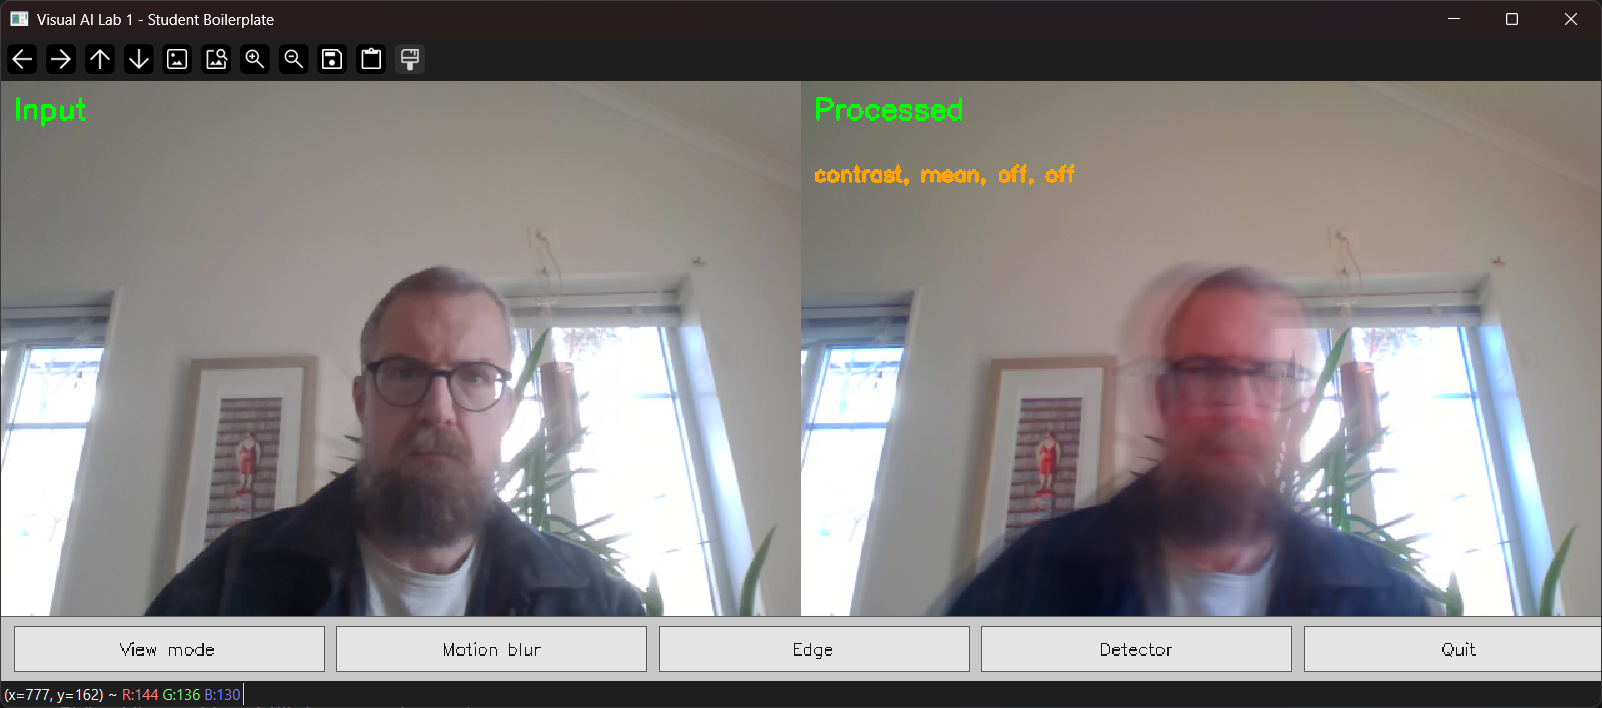
\includegraphics[width=\linewidth,height=0.38\textheight,keepaspectratio]{g1.png}
    \end{column}
    \begin{column}{0.48\textwidth}
      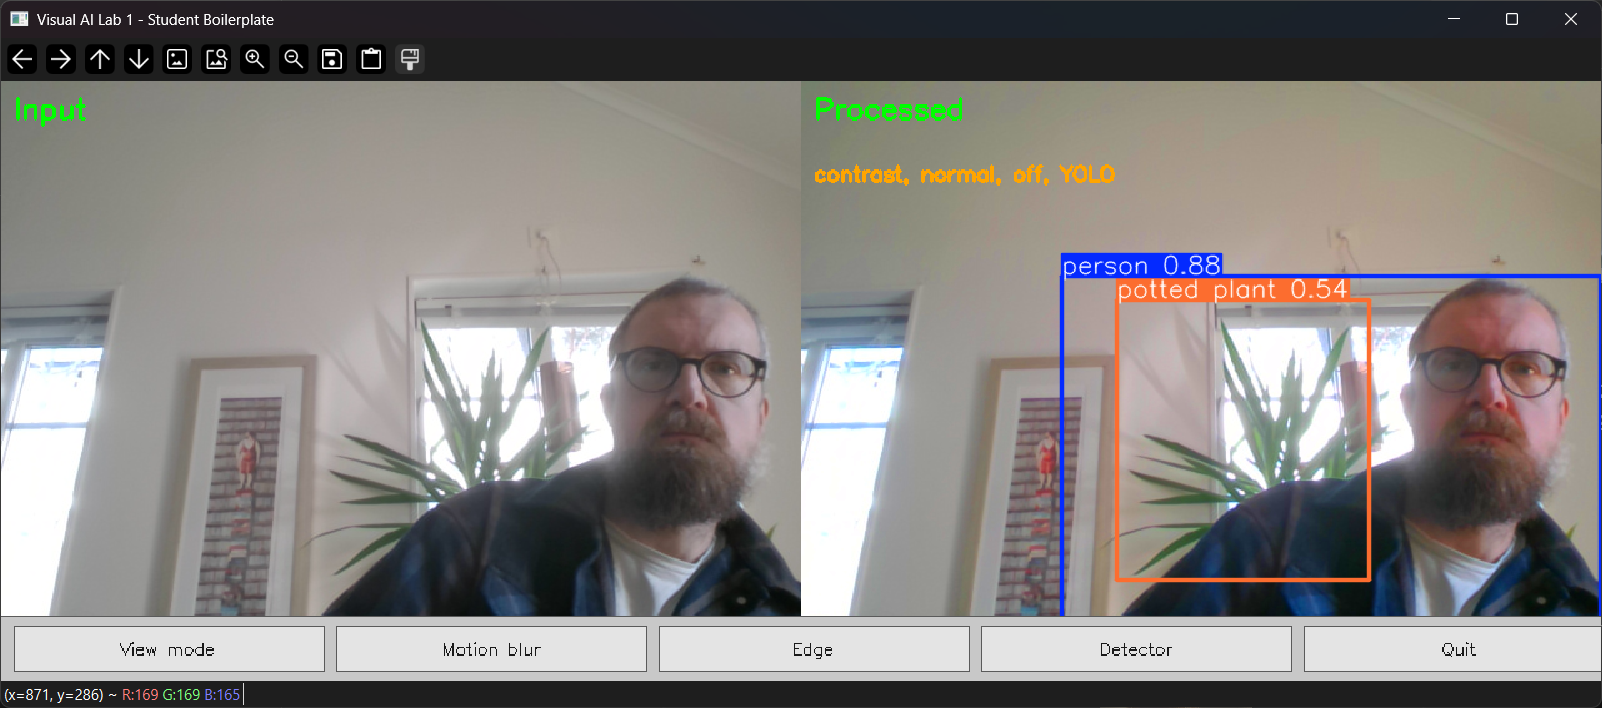
\includegraphics[width=\linewidth,height=0.38\textheight,keepaspectratio]{g2.png}
    \end{column}
  \end{columns}
\end{frame}

\begin{frame}{Failure case}
  \textbf{Scenario:} heavy motion blur.
  \begin{itemize}
    \item YOLO cannot detect objects after edge detection.
  \end{itemize}
  \vspace{0.25em}
  \begin{center}
    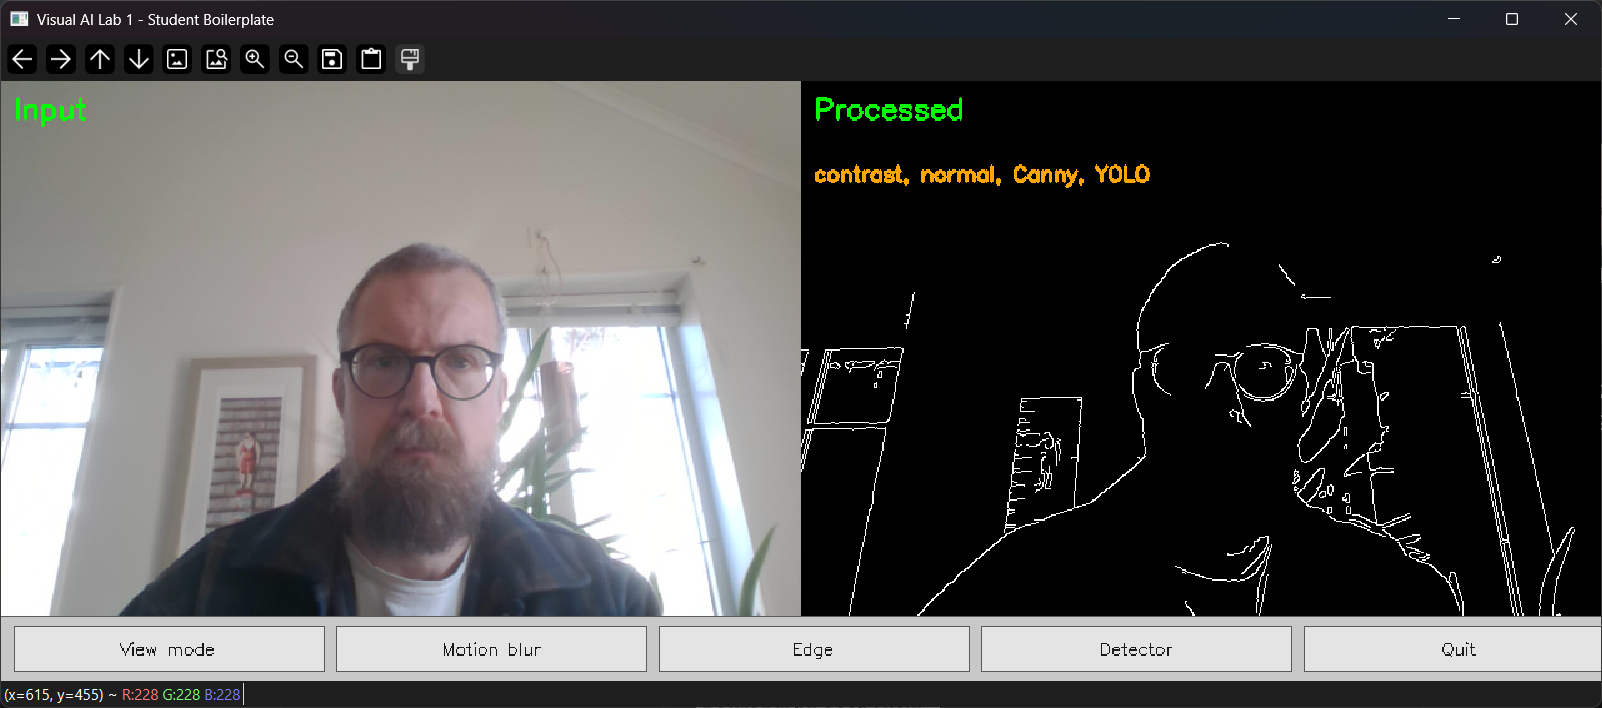
\includegraphics[width=0.88\linewidth,height=0.42\textheight,keepaspectratio]{b1.png}
  \end{center}
\end{frame}

\section{Analysis and Limitations}

\begin{frame}{Works and fails}
  \textbf{Why it works}
  \begin{itemize}
    \item \textbf{Modular order} makes behavior inspectable.
    \item \textbf{Pretrained detectors} encode broad visual priors. No provisioning for training.
    \item \textbf{Classical stages} are fast and deterministic for demos (grayscale, Canny, Sobel).
  \end{itemize}

  \textbf{Why it fails}
  \begin{itemize}
    \item \textbf{Latency / resources:} R-CNN on CPU is slow. YOLO is lighter but still sensitive to blur and resolution.
    \item \textbf{Composition:} stacking operations can compound artifacts (e.g.\ temporal blur then edges). \textbf{Also, YOLO is not very good at detecting small objects.}
    \item \textbf{Running:} tricky to get right versions of libraries.
    \item Annoying that the windows close button (X) does not work. Quit button or \texttt{q}/\texttt{Esc} works instead.
  \end{itemize}
\end{frame}

\section{Key Takeaways}

\begin{frame}{Key takeaways}
  \begin{itemize}
    \item Vision systems are \textbf{pipelines}: early stages constrain what later stages see.
    \item \textbf{Classical vs learned:} edges and color transforms explain structure cheaply. Detectors generalize but need sensible inputs and compute.
    \item \textbf{Evaluation is visual:} side-by-side comparison makes success and failure modes obvious.
    \item \textbf{OpenCV:} easy to use due to the many examples on the internet.
  \end{itemize}
\end{frame}

\end{document}
